% -----------------------------------------------------------------------------
%   Arquivo: ./01-texto/desenvolvimento.tex
% -----------------------------------------------------------------------------


\section{Desenvolvimento}\label{sec:desenvolvimento}	% edite para alterar o título da seção

Implementou-se em linguagem python uma abstração de uma rede social, contendo indivíduos e conexões entre os mesmos.

Para isso, criou-se uma classe Individuo (para representar um individuo da rede social), contendo somente dois atributos: id e profissão, ambos do tipo inteiro.

\begin{center}
  \captionof{figure}{Classe Individuo}
  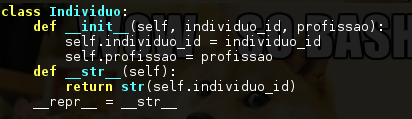
\includegraphics[scale=0.45]{./02-figuras/individuo.png}
  \label{fig:patoA}
\end{center}

Cada individuo tem uma profissão e para esta simulação, foram definidas 5 profissões possíveis:

\begin{center}
  \captionof{figure}{Profissões Possíveis}
  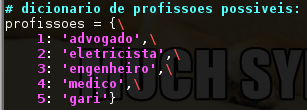
\includegraphics[scale=0.45]{./02-figuras/profissoes.png}
  \label{fig:patoA}
\end{center}


Neste problema, definiu-se que a rede social simulada terá 20 individuos. Para isso, foi criada uma lista de individuos:

\begin{center}
  \captionof{figure}{Lista de Individuos}
  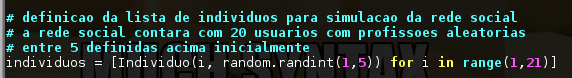
\includegraphics[scale=0.35]{./02-figuras/lista_individuos.png}
  \label{fig:patoA}
\end{center}

A rede social com seus indivíduos e suas amizades foi expressa como um grafo bi direcional e implementada utilizando-se a estrutra de dados dict (dicionário) nativa da linguagem python. Essa estrutura de dados consiste em uma tabela do tipo Chave-Valor, onde ela retorna os valores de uma determinada chave. Um grafo com vários vértices e arestas é bem representado pela estrutura dict, pois seus vértices são as chaves do dicionário e os valores dessas chaves são os vértices adjacentes a ela, representado assim as arestas do grafo.

\begin{center}
  \captionof{figure}{Implementação inicial da Rede Social}
  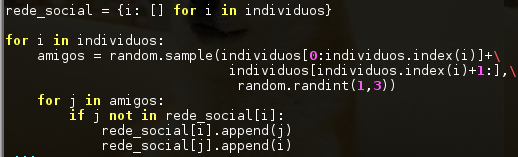
\includegraphics[scale=0.35]{./02-figuras/dict.png}
  \label{fig:patoA}
\end{center}


A primeira abordagem foi a geração aleatória de amizades entre individuos e inserção dessas amizades na rede social. Uma rede aleatória foi gerada e visualizada mediante o auxílio da ferramenta vis. 
A \textbf{Figura \ref{fig:patoB}} representa a visualização gerada.

\begin{figure*}
	\centering
	\caption{Visualização da Rede Social} 
	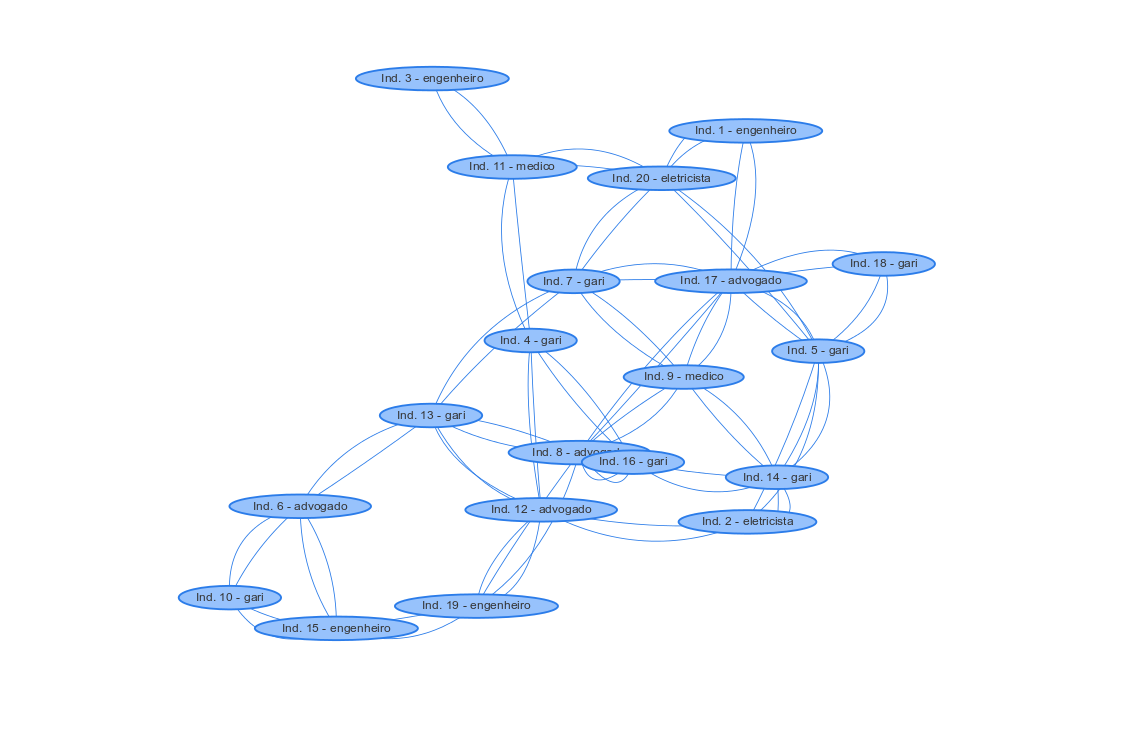
\includegraphics[scale=0.4]{./02-figuras/vis.png}
	\label{fig:patoB}
\end{figure*}

Após essa rede ter sido gerada, substituiu-se a geração aleatórias de redes sociais por essa rede gerada, para facilitar a simulação e consequentemente a validação dos resultados obtidos.

Tendo-se a rede social gerada (e consequentemente um grafo), desenvolveu-se a busca de prestadores de serviço à partir de um indivíduo, seus amigos e os amigos de seus amigos.

Para isso, implementou-se a função profissionais, que recebe como parâmetros g (rede social), individuo e profissão desejada. A função realiza uma busca de profundidade limitada ao segundo nível alcançável pelo indivíduo no grafo g e retorna todos os individuos alcançáveis até o segundo nível que atendem à profissão desejada.

A busca em profundidade limitada usa a mesma técnica da busca em profundidade, de utilizar-se uma pilha para visitação dos nodos, só que com a limitação do nível da busca, ela não permite que os nós abaixo do segundo nível sejam inseridos na pilha.

A \textbf{Figura \ref{fig:patoA}} mostra a implementação da função profissionais

\begin{figure*}
	\centering
	\caption{profissional - Função que realiza DLS até o nível 2 de um indivíduo da rede social e retorna indivíduos que prestam o serviço desejado} 
	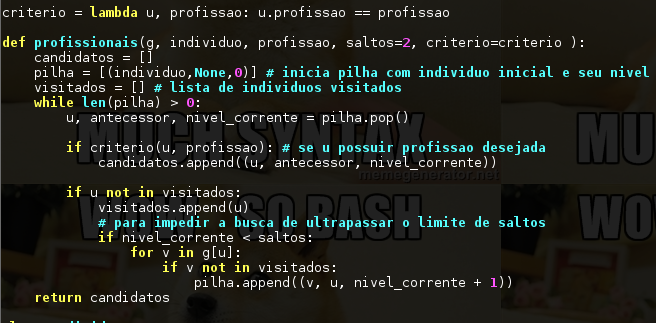
\includegraphics[scale=0.4]{./02-figuras/profissionais.png}
	\label{fig:patoA}
\end{figure*}
